\documentclass[12pt,a4paper]{article}
\usepackage{setspace}
\doublespacing
\usepackage{hyperref}
\hypersetup{
	colorlinks,
	citecolor=black,
	filecolor=black,
	linkcolor=black,
	urlcolor=black
}
\usepackage[]{times}
\usepackage[latin1]{inputenc}
\usepackage{amsmath}
\usepackage{amsfonts}
\usepackage{amssymb}
\usepackage{makeidx}
\usepackage{graphicx}
\begin{document}
	
	\title{Web Security Application}
	\author{Becker, Joshua\\ Okereke, Uchechukwu Okpo\\ Shama, Muthuraman Venkatesan\\ Ulbrich, Damian}
	\date{\today}
	\maketitle
	\clearpage
	
	
	\tableofcontents
	\clearpage
	
	\section{Introduction}
	
	
	\begin{flushleft}
	Since the creation of the Internet, the world has seen it evolve with lots of practical applications. These include things like eCommerce, Instant Messaging, Video Streaming services and the likes. With this evolution and advancements, there has also been a rise in misuse and security concerns regarding identity theft, private data leaks etc.
	
		
	One subset of eCommerce that is ever so popular is Online shopping, allowing consumers to directly buy goods or services from a seller over the Internet using a web browser. Consumers find a product of interest by visiting the website of the retailer directly or by searching among alternative vendors using a shopping search engine, which displays the same product's availability and pricing at different e-retailers. Customers must have access to the Internet and a valid method of payment in order to complete a transaction, such as a credit card, an Interac-enabled debit card, or a service such as PayPal. Hence, the element of security for user details is crucial.
	
	
	In this project, we were tasked to create a simple eCommerce site called Webshop. We look to see how a user can interact with the online store and be able to make purchases with or without registering on the site while being safeguarded against security attacks. This report, documents the required specifications of the project, alongside how the requirements were implemented. Also, the challenges encountered during the course of the project.
	
	
	\end{flushleft}
	\section{Project Specification}
	
		\subsection{Secure Session handling with Cookies and database}
		
		\subsection{Timeout for Session and Tokens}
		
		\subsection{Secure Storage of passwords}
		
		\subsection{CSRF handling}
		
			\begin{flushleft}
				Cross-site request forgery, also known as one-click attack or session riding and abbreviated as CSRF (sometimes pronounced sea-surf) or XSRF, is a type of malicious exploit of a website where unauthorized commands are transmitted from a user that the web application trusts. There are many ways in which a malicious website can transmit such commands; specially-crafted image tags, hidden forms, and JavaScript XMLHttpRequests, for example, can all work without the user's interaction or even knowledge. Unlike cross-site scripting (XSS), which exploits the trust a user has for a particular site, CSRF exploits the trust that a site has in a user's browser.
			\end{flushleft}
			
		\subsection{XSS handling}
		
			\begin{flushleft}
				Cross-site scripting (XSS) is a type of computer security vulnerability typically found in web applications. XSS enables attackers to inject client-side scripts into web pages viewed by other users. A cross-site scripting vulnerability may be used by attackers to bypass access controls such as the same-origin policy. 
			\end{flushleft}
			
		\subsection{SQL-injection handling}
		
		\subsection{Secure logic design}
		 
	 	
	\section{Problem Analysis}
	
	\section{Implementation}
		
	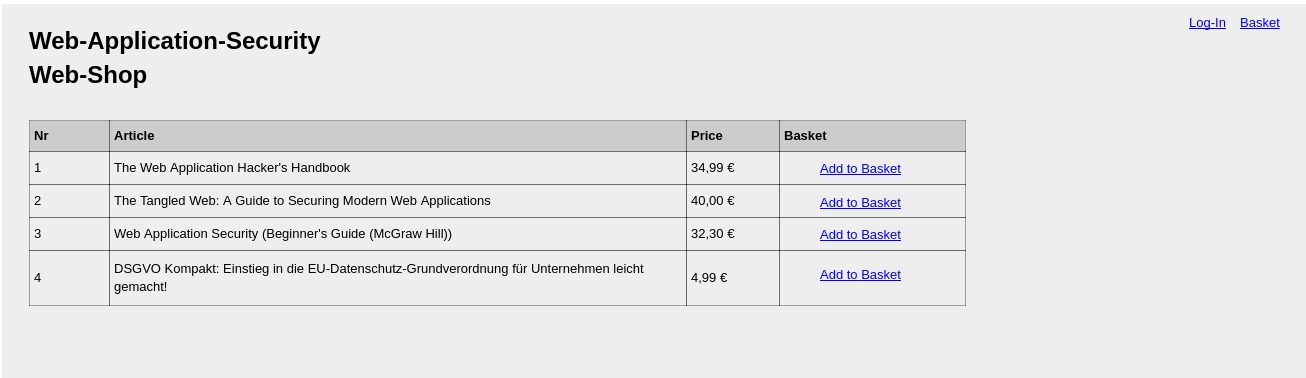
\includegraphics[scale = 0.5]{index}
	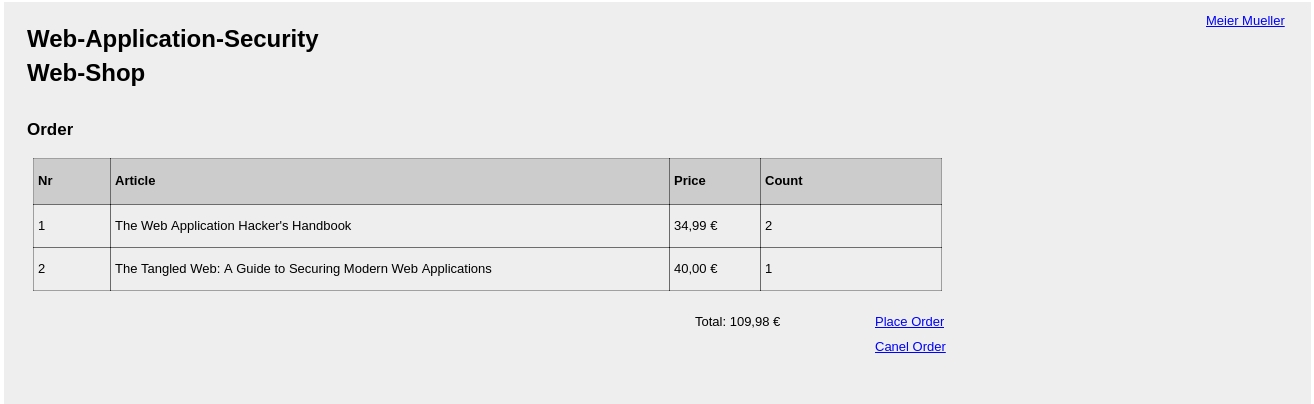
\includegraphics[scale = 0.5]{order}
	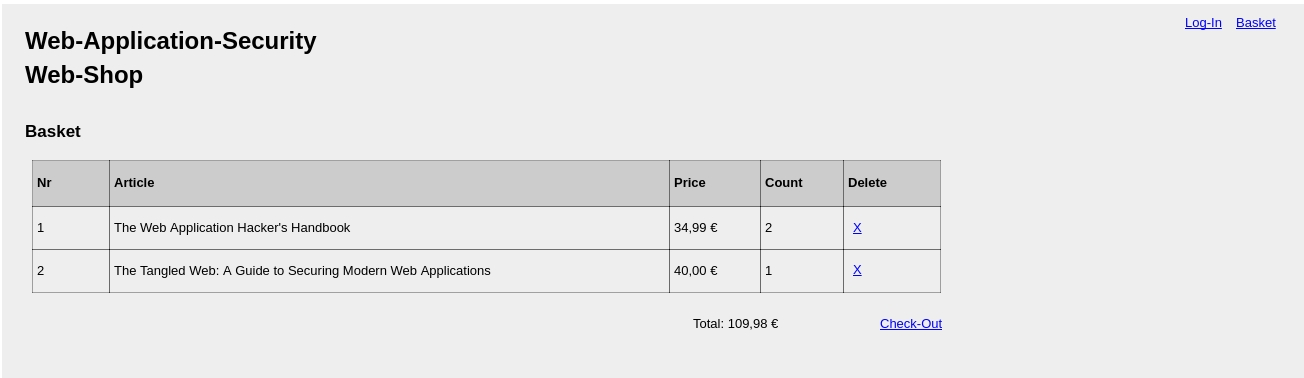
\includegraphics[scale = 0.5]{basket}
	
	\section{Conclusion and Lessons Learnt}
\end{document}